% !TeX spellcheck = en_US 
\documentclass{article}
\usepackage[paper=a4paper, left=2.5cm, right=2.5cm, top=2.5cm, bottom=2.5cm]{geometry}
\usepackage[section]{placeins}
\usepackage[indent=0cm]{parskip}
\usepackage[colorlinks, linkcolor=blue, urlcolor=magenta, citecolor=teal, bookmarks]{hyperref}

\usepackage{pack}
\usepackage{pack-notebook}

\title{
  {\Huge Notebook on the \textit{Colloquio}} \\
  \colloquioTitle
}

\author{
  \myFullName \\
  {\small Advisor: \advisorFullName}
}

\date{\colloquioDate}

\begin{document}
  \maketitle
  \begin{abstract}
    I'm writing this document for my personal use. It's a collection of notions,
    definitions, reflections, and more, produced as I worked on the \textit{colloquio}.
    I hope that this will help me during the preparation of the talk!
  \end{abstract}
  \tableofcontents
  \clearpage
  
  \part{Theoretical foundation}
  \section{The model}
  Restricted Boltzmann Machines are a model used mainly for unsupervised learning. We collect
  data from an unknown distribution and then use it to set the parameters of the RBM to match
  the starting distribution as closely as possible.
  
  \subsection{General RBM}
  Consider a fully-connected bipartite undirected graph as shown in Figure~\ref{fig:generalRBM}.
  It consists of \emph{visible} layer with $m$ nodes labeled by \(V_1, \dots, V_m\) and a
  \emph{hidden} layer whose \(n\) nodes are labeled by \(H_1, \dots, H_n\). We call \(\mathcal{V}\)
  the set of visible nodes, and \(\mathcal{H}\) the set of hidden nodes.
  \begin{figure}
    \centering
    \resizebox{0.5\textwidth}{!}{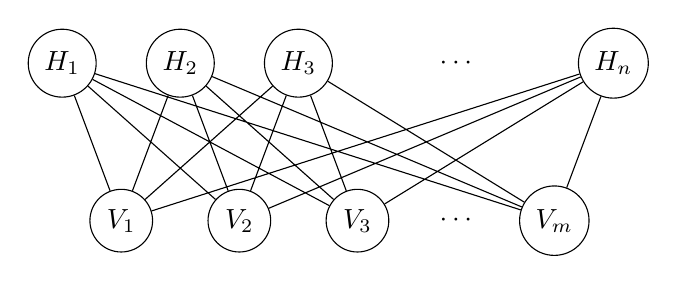
\begin{tikzpicture}%[node distance={15mm}, thick, main/.style = {draw, circle}] 
  \node[draw, circle] (h1) at (1.5,1)   {$H_1$}; 
  \node[draw, circle] (h2) at (3,1)   {$H_2$};
  \node[draw, circle] (h3) at (4.5,1)   {$H_3$};
  \node            (hdots) at (6.5,1) {$\cdots$};
  \node[draw, circle] (hn) at (8.5,1)   {$H_n$};
  
  \node[draw, circle] (v1) at (2.25,-1)   {$V_1$}; 
  \node[draw, circle] (v2) at (3.75,-1)   {$V_2$};
  \node[draw, circle] (v3) at (5.25,-1)   {$V_3$};
  \node            (vdots) at (6.5,-1) {$\cdots$};
  \node[draw, circle] (vm) at (7.75,-1)   {$V_m$};
  
  \draw (v1)--(h1)
        (v1)--(h2)
        (v1)--(h3)
        (v1)--(hn)
        (v2)--(h1)
        (v2)--(h2)
        (v2)--(h3)
        (v2)--(hn)
        (v3)--(h1)
        (v3)--(h2)
        (v3)--(h3)
        (v3)--(hn)
        (vm)--(h1)
        (vm)--(h2)
        (vm)--(h3)
        (vm)--(hn);
\end{tikzpicture} }
    \caption{An RBM graph with \(n\) hidden and \(m\) visible nodes.}
    \label{fig:generalRBM}
  \end{figure}
  Let us consider a random variable \(X_U\) associated with a node \(U\) (either visible or hidden)
  that takes values in \(\Lambda_U\). We say that our graph satisfies the \emph{Markov
  property} if 
  \begin{align*}
    \CondProb{X_v}{\{X_{v'}\}_{v'\in (\mathcal{V} \setminus \{v\})}, \{X_h\}_{h\in \mathcal{H}}} =
    \CondProb{X_v}{\{X_h\}_{h\in \mathcal{H}}}, \\
    \CondProb{X_h}{\{X_v\}_{v\in \mathcal{V}}, \{X_{h'}\}_{h'\in (\mathcal{H} \setminus \{h\})}} =
    \CondProb{X_h}{\{X_v\}_{v\in \mathcal{V}}}.
  \end{align*}
  or saying it simpler: a visible node is independent of all other visible nodes,
  and the same for hidden ones. The graph structure is telling us the dependencies between
  the random variables: if 2 nodes are not connected their associated variables are independent.
  We will assume that \(\Lambda_v = \Lambda_{v'} \,\, \forall v,v' \in \mathcal{V}\) and analog
  for the hidden variables. For simplicity we use the notation
  \[\prob{\vec{v}, \vec{h}} = \Prob{X_{V_i} = v_i, X_{H_j} = h_j
                                    \quad\forall i \in \{1,\dots,m\}, \forall j \in \{1,\dots,n\}}.\]
  
  
  It follows from \emph{Hammersley-Clifford Theorem}\cite{fischer2012introduction} that 
  \begin{equation} \label{eq:hammersley-clifford-thm}
    \prob{\vec{v}, \vec{h}} = \frac{1}{Z} \prod_{i=1,j=1}^{m,n} \psi_{i,j}(v_i, h_j),
  \end{equation}
  where
  \[Z = \sum_{\vec{v}, \vec{h}}\prod_{i=1,j=1}^{m,n} \psi_{i,j}(v_i, h_j)\]
  is called \emph{partition function} and \(\psi_{i,j}\) are called \emph{potential functions}.
  The equation~\eqref{eq:hammersley-clifford-thm} can be written in a more convenient way as
  \begin{equation} \label{eq:RBMdistribution}
    \prob{\vec{v}, \vec{h}} 
      = \frac{1}{Z} \exp\left(\sum_{i=1,j=1}^{m,n}\log\left(\psi_{i,j}(v_i, h_j)\right)\right)
      = \frac{1}{Z} \exp\left(-E(\vec{v}, \vec{h})\right)
  \end{equation}
  where \(E(\vec{v}, \vec{h})=-\sum_{i=1,j=1}^{m,n}\log\left(\psi_{i,j}(v_i, h_j)\right)\) is called
  \emph{energy function}. It should be clear the link with statistical mechanics since equation~\eqref{eq:RBMdistribution}
  is a \emph{Boltzmann distribution} where \(\beta\) (inverse of the temperature) is set to 1. 
  We can go further with the physical interpretation observing that there could be ``interaction''
  only between nodes of different layers, so only when nodes are directly connected: the graph
  structure is again useful to understand RBMs.
  
  The division between visible and hidden nodes is used because only the visible one represents the
  features of the goal distribution; the hidden nodes can be thought of as hidden features that
  the model learns during training. Given this context, it's particularly important the marginal
  distribution
  \[\prob{\vec{v}} = \sum_{\vec{h}} \prob{\vec{v},\vec{h}}.\]
  The Markov property above easily imply this relations on conditional probabilities
  \[
    \condprob{\vec{h}}{\vec{v}} = \prod_{j=1}^n \condprob{h_j}{\vec{v}} \quad\text{and}\quad
    \condprob{\vec{v}}{\vec{h}} = \prod_{i=1}^m \condprob{v_i}{\vec{h}}.
  \]
  
  We empathize that the energy function must be sum of functions of at most 2 nodes;
  the most general energy for an RBM is
  \begin{equation} \label{eq:energyRBM}
    E(\vec{v}, \vec{h}) = \sum_{i}^m f_i{(v_i)} + \sum_{j}^n g_j{(h_j)} +
                          \sum_{i=1,j=1}^{m,n} I_{i,j}{(v_i,h_j)}
  \end{equation}
  
  \subsubsection{Maximum Likelihood}
  We suppose that the energy depends on a set of parameters \(\vec{\theta}\), so it is the function
  \(E(\vec{v}, \vec{h};\vec{\theta})\); obviously also all the other objects of the RBM depend on these parameters. The standard way of estimating parameters in a statistical
  model is maximizing the likelihood. Suppose that our \emph{training set} is 
  \(S = \left\{\vec{\bar{v}}_k\right\}_{k \in \{1,\dots,\ell\}}\) so that the likelihood
  \begin{align*}
    \log\likelihood{\vec{\theta}}{S}
      &= \sum_{k=1}^\ell \log\left(\prob{\vec{\bar{v}}_k;\vec{\theta}}\right)
       = \sum_{k=1}^\ell \log\left(\sum_{\vec{h}} 
                                      \exp\left[-E(\vec{\bar{v}}_k,\vec{h};\vec{\theta})\right]\right)
         -\ell \log{Z(\vec{\theta})} \\
      &= \sum_{k=1}^\ell \log\left(\sum_{\vec{h}} 
                                      \exp\left[-E(\vec{\bar{v}}_k,\vec{h};\vec{\theta})\right]\right)
         -\ell \log\left(\sum_{\vec{v},\vec{h}} 
                                 \exp\left[-E(\vec{v},\vec{h};\vec{\theta})\right]\right)
   \end{align*}
   where we used the \(\log\) since it's a monotonic function and does not change the maximum position.
  Let's compute the gradient (we drop both the sum on \(S\) since the likelihood it's linear and the dependence from \(\vec{\theta}\))
  \begin{align*} \displaystyle
    \ParDer{\log\likelihood{\vec{\theta}}{\vec{\bar{v}}}}{\vec{\theta}}
      &= -\frac{1}{\sum_{\vec{h}}\exp\left[-E(\vec{\bar{v}},\vec{h})\right]}
          \sum_{\vec{h}}\exp\left[-E(\vec{\bar{v}},\vec{h})\right]
          \ParDer{E(\vec{\bar{v}},\vec{h})}{\vec{\theta}}+ \\
      &\quad +\frac{1}{\sum_{\vec{v},\vec{h}}\exp\left[-E(\vec{v},\vec{h})\right]}
          \sum_{\vec{v},\vec{h}}\exp\left[-E(\vec{v},\vec{h})\right]
          \ParDer{E(\vec{v},\vec{h})}{\vec{\theta}} \\
      &= -\sum_{\vec{h}}\condprob{\vec{h}}{\vec{\bar{v}}}
        \ParDer{E(\vec{\bar{v}},\vec{h})}{\vec{\theta}} +
        \sum_{\vec{v},\vec{h}}\prob{\vec{v},\vec{h}}
        \ParDer{E(\vec{v},\vec{h})}{\vec{\theta}} =\\
      &= -\ExpVal{\condprob{\vec{h}}{\vec{\bar{v}}}}{\ParDer{E(\vec{\bar{v}},\vec{h})}{\vec{\theta}}}
         +\ExpVal{\prob{\vec{v},\vec{h}}}{\ParDer{E(\vec{v},\vec{h})}{\vec{\theta}}}
  \end{align*}
  
  Until now we haven't used the fact that the RBM is a bipartite graph and what we said on likelihood
  hold also for general graph topologies\footnote{See \cite{fischer2012introduction} for \emph{Markov
  Random Fields}}.
  We recall that for RBMs the energy must have the form \eqref{eq:energyRBM} and the parameters \(\vec{\theta}\) are the union of parameters on single functions \(f_i\), \(g_j\), and \(I_{i,j}\).
  Using these facts, and calling \(\vec{\theta}_{i,j}\) the parameters of the function \(I_{i,j}\)
  \[
    \ParDer{\log\likelihood{\vec{\theta}}{\vec{\bar{v}}}}{\vec{\theta}_{i,j}} 
      = -\ExpVal{\condprob{h_j}{\vec{\bar{v}}}}{\ParDer{I_{i,j}(\bar{v}_i,h_j)}{\vec{\theta}_{i,j}}}
        +\ExpVal{\prob{v_i,h_j}}{\ParDer{I_{i,j}(v_i,h_j)}{\vec{\theta}_{i,j}}}.
  \]
  Analogously if \(\vec{\theta}_i\) and \(\vec{\theta}_j\) are the parameters of the functions
  \(f_i\) and \(g_j\) respectively
  \begin{align*}
    \ParDer{\log\likelihood{\vec{\theta}}{\vec{\bar{v}}}}{\vec{\theta}_i} 
    &= -\ParDer{f_i(\bar{v}_i)}{\vec{\theta}_i}
       +\ExpVal{\prob{v_i}}{\ParDer{f_i(v_i)}{\vec{\theta}_i}}, \\
    %
    \ParDer{\log\likelihood{\vec{\theta}}{\vec{\bar{v}}}}{\vec{\theta}_j} 
    &= -\ExpVal{\condprob{h_j}{\vec{\bar{v}}}}{\ParDer{g_j(h_j)}{\vec{\theta}_i}}
       +\ExpVal{\prob{h_j}}{\ParDer{g_j(h_j)}{\vec{\theta}_j}}.
  \end{align*}
  Despite the gradient formulas seem simple, calculating the expected values is computationally
  untreatable and some approximations are needed. Training algorithms for RBM are just a clever way
  of computing an approximation of these gradients.
  
  \subsection{Binary Classic RBM} \label{subsec:binary-classic-RBM}
  Binary RBM is the simpler form of RBM, but still, they are quite powerful.
  They are obtained by choosing
  \[\Lambda_V = \Lambda_H = \{0,1\},\]
  \[
    f_i(x) = -b_ix, \quad g_j(y) = -c_jy  \quad\text{and}\quad I_{i,j}(x,y)=-w_{i,j}xy.
  \]
  It's not difficult to prove these relations\footnote{The proof can be found on
  \cite{fischer2012introduction}, pages 24-25.}
  \begin{align}
    \label{eq:prob-one-hidden-given-visible}
    \condprob{h_j=1}{\vec{v}} &= \sigmoid{\sum_{i=1}^m w_{i,j}v_i+c_j},\\
    \label{eq:prob-one-visible-given-hidden}
    \condprob{v_i=1}{\vec{h}} &= \sigmoid{\sum_{j=1}^n w_{i,j}h_j+b_i}.
  \end{align}
  Observing that for binary variables \(\ExpVal{\prob{v}}{v} = \prob{v=1}\), the gradient of
  the likelihood takes the nice form
  \begin{align}
    % gradient of w_{i,j}
    \nonumber
    \ParDer{\log\likelihood{\vec{\theta}}{\vec{\bar{v}}}}{w_{i,j}}
      &= \bar{v}_i\ExpVal{\condprob{h_j}{\vec{\bar{v}}}}{h_j} 
         -\ExpVal{\prob{\vec{v}}}{\ExpVal{\condprob{h_j}{\vec{v}}}{v_ih_j}} \\
      \label{eq:logL-gradient-w-RBM}
      &= \bar{v}_i \sigmoid{\sum_{i'=1}^m w_{i',j}\bar{v}_{i'}+c_j}
         -\ExpVal{\prob{\vec{v}}}{v_i \sigmoid{\sum_{i=1}^m w_{i',j}v_{i'}+c_j}} \\
    % gradient of b_i
    \ParDer{\log\likelihood{\vec{\theta}}{\vec{\bar{v}}}}{b_i}
      &= \bar{v}_i -\ExpVal{\prob{\vec{v}}}{v_i} \\
    % gradient of c_j
    \ParDer{\log\likelihood{\vec{\theta}}{\vec{\bar{v}}}}{c_j}
      &= \sigmoid{\sum_{i=1}^m w_{i',j}\bar{v}_{i'}+c_j}
         -\ExpVal{\prob{\vec{v}}}{\sigmoid{\sum_{i=1}^m w_{i',j}v_{i'}+c_j}}
  \end{align}
  \ExplainBox{Why all the formulas contains an expected value on \(\prob{\vec{v}}\)?}{
    Essentially because it's convenient when implementing the training algorithms.
    
    Since we have to figure out a way to sample complex distributions, it's better to have
    only one instead of one different for each node. For example, for the derivative with
    respect to \(c_j\) we have to take the expected value on the distribution \(\prob{h_j}\), but using the fact
    \(\sum_{\vec{v}}\prob{\vec{v}}=1\)
    \begin{align*}
      \ExpVal{\prob{h_j}}{h_j} & = \sum_{h_j}\prob{h_j}h_j 
         = \sum_{h_j}\sum_{\vec{v}}\condprob{h_j}{\vec{v}}\prob{\vec{v}} h_j                                           \\
                               & = \sum_{\vec{v}}\prob{\vec{v}}\sum_{h_j}\condprob{h_j}{\vec{v}} h_j 
         = \sum_{\vec{v}}\prob{\vec{v}}\ExpVal{\condprob{h_j}{\vec{v}}}{h_j} \\
                               & = \ExpVal{\prob{\vec{v}}}{\ExpVal{\condprob{h_j}{\vec{v}}}{h_j}},
    \end{align*}
    we obtained an expected value respect \(\prob{\vec{v}}\). We are lucky because
    in Classic Binary RBM the other expected value can be computed analytically in
    an easy way\footnote{Well, it's not fortune... Classic binary RBMs are so important
    because of this little trick that makes training far easier than other BMs
    \& RBMs.}.
  }
  \section{Classical Training Algorithms}
  All classic training algorithms for RBM are based on the likelihood maximization,
  using a recurrent gradient ascent, based on formulas from Section \ref{subsec:binary-classic-RBM}.
  As already noted the formulas contain some expected values calculation over the
  entire Boltzmann distribution of the visible layer, the is untreatable exactly,
  and requires some approximations.
  Before going through the methods, we first present the general learning formula for 
  following gradient,  that includes some extra terms that improve the algorithm.
  
  \subsection{General update rule for gradient ascent}
  Let \(\vec{\theta}^{(t)}\) the parameters of the model after \(t\) step of the update.
  The update formula for a single training data \(\vec{\bar{v}}\) is given by
  \[
    \vec{\theta}^{(t+1)} = \vec{\theta}^{(t)}
                           \underbrace{
                             + \eta \ParDer{\log\likelihood{\vec{\theta}}{\vec{\bar{v}}}}{\vec{\theta}}
                             - \lambda \vec{\theta}^{(t)}
                             + \nu \Delta\vec{\theta}^{(t-1)}
                           }_{\coloneqq \Delta\vec{\theta}^{(t)}}
  \]
  where \(\eta,\lambda,\nu \in \mathbb{R}^+\) are respectively the \emph{learing rate},
  the \emph{weight decay parameter} and \emph{momentum parameter}.
  All of them are meta-parameters of the algorithm and doesn't not to be constant all
  over the learning.
  
  We now see a brief explanation on what this parameters are. For a much more detailed one
  see \cite{hinton2012practical}, where is explained  also how to tune them.
  \subsubsection{Learing rate}
  It is ``how much the model is influenced by the data''. It should be larger the beginning to
  explore a wider region of space, and decrease over time.
  \subsubsection{Weight decay}
  A physical explanation of this term, that makes ``little''parameters preferred, is that
  bigger values in the energy could also be interpreted as system in low temperature
  \footnote{In Boltzmann distribution if all the energy take a factor is the same as
  the temperature reduced by the same factor.}. The system in low temperature means that
  essentially only low energy states are possible and, in the language of ML, there's overfitting,
  since the algorithm train the system to have energy minimum in the training set.
  
  The weight decay can be interpreted as adding the term \(-\lambda\frac{\left|\vec{\theta}\right|^2}{2}\)
  to the likelihood and only after this take the gradient to follow.
  \subsubsection{Momentum}
  This is a term to eliminate the effect of the outliers. When following the gradient,
  the moving gain some pace that can is used to move through some annoying points that
  behaves differently from the average on their neighborhood. Another way to say it is
  ``the momentum makes the manifold of the gradient smoother''.
  
  \subsubsection{Batches}
  The training data contains many value \(\vec{\bar{v}}_k\). Update the parameters of a model
  after every computation of the gradient given a single training data is too slow but
  especially subject to large fluctuations caused by outliers. On the other hand, change
  parameters after updates for every point are computed will be not good as well.
  
  The solution to this problem are the \emph{batches}. The data is partitioned in small sets
  and only after that the gradients of all the data in the batch were computed, the parameters
  are updated. The size of the batches is a meta-parameter of the training algorithm, in 
  the reference \cite{hinton2012practical} there are many insights on how use batches smoothly.
  
  
  \subsection{Naive Gibbs Sampling}
  The idea is simple: to estimate the expected values we set up a
  Markov Chain with invariant distribution equal to \(\prob{\vec{v}}\).
  If we wait enough steps, the Markov chain is sampling from the 
  invariant distribution and we can use these sample to extimate the
  expected values.
  
  Note that not all Markov chains have an invariant distribution, and even if they do,
  it is not certain that they will converge on it. In \cite{fischer2012introduction} there's 
  a great discussion on Markov chains and their properties.
  
  This algorithm belong to the class named \emph{Markov Chain MonteCarlo algorithms}.
  
  \subsubsection{Gibbs Sampling in general}
  We first describe the general idea of Gibbs sampling, without the proofs of correctness.
  Let's suppose to have a multivariate distribution \(\pi{(\vec{x})}\), with \(\vec{x}\) a
  generic vector of random variables, and we would like to sample it.
  We say that \(\dim{\vec{x}} = n\) and we will use \(\vec{x}_{-i}\) to indicate the vector
  \(\vec{x}\) with the entry \(x_i\) removed.
  We setup a Markov chain where states are all possible values of \(\vec{x}\), and transition
  probability is given by
  \[
    \prob{\vec{x} \to \vec{y}} = 
      \begin{cases}
        q{(i)} \pi{(y_i|\vec{x}_{-i})} &
          \text{if } \exists i \in \{1,\dots,n\} \text{ so that: } j\neq i \implies x_j = y_j\\
        0 &\text{otherwise}
      \end{cases}.
  \]
  Here \(q{(i)}\) is a distribution over \(\{1,\dots,n\}\), that chooses which component is
  updated. In most of the cases there is no reason to pick \(q\) different from the uniform
  distribution. Note that there are many ways (\(n\), to be precise) to realize \(\vec{x} = \vec{y}\),
  so in practice we have 
  \[
    \prob{\vec{x} \to \vec{x}} = \sum_{i=1}^{n} q{(i)} \pi{(x_i|\vec{x}_{-i})}.
  \]
  
  The transition matrix above is equivalent to use the Algorithm~\ref{alg:gibbs-sampling-general}.
  
  \begin{algorithm}[H]
    \DontPrintSemicolon
    \SetKwInOut{Input}{Input}\SetKwInOut{Output}{Output}
    
    \Input{goal distribution \(\pi{(\vec{x})}\), Markov Chain current state \(\vec{x}\),
           distribution \(q{(i)}\)}
    \Output{Markov Chain next state \(\vec{y}\)}
    
    init \(a\), \(\vec{y}\), \(i\)\;
    \(i \leftarrow \text{ sample } q{(\cdot)}\)\;
    \( y_i \leftarrow \pi{(\cdot|\vec{x}_{-i})}\)\;
    \For{\(j\in \{1,\dots,n\},\, j\neq i\)}{
      \(y_j \leftarrow x_j\)\;
    }
    
    \caption{update of the Markov Chain in Gibbs sampling.}
    \label{alg:gibbs-sampling-general}
  \end{algorithm}
  \ExplainBox{Why does this algorithm work good?}{
    A key hypothesis need to make this algorithm functional is knowing how to sample from
    \(\pi{(y_i|\vec{x}_{-i})}\) in an efficient way. If the conditional probability can't be
    computed without knowing how to sample from \(\pi{(\vec{x})}\) the algorithm is useless.
    
    \begin{example}
      If \(\pi{(\vec{x})} \propto \prod_{i=1}^n \exp{[-x_i^2]}\), then \(\pi{(y_i|\vec{x}_{-i})}\)
      is simply a 1D Gaussian with an appropriate variance, easy to sample.
    \end{example}
  }
  There are many different variants of Gibbs Sampling. The most common is \emph{period Gibbs sampling}
  where the variable to be updated is not chosen at random based on a distribution \(q\) but
  subsequently in fixed predefined order. 
  
  
  \subsubsection{Gibbs Sampling on Binary Classic RBM}
  The first thing to say is that we are interested in \(\prob{\vec{v}}\), but it's easier to work
  with \(\prob{\vec{v},\vec{h}}\) and then restrict the sample only on the visible layer.
  
  As second point we remind that
  \[
    \condprob{v_i}{\vec{v}_{-i},\vec{h}} = \condprob{v_i}{\vec{h}},
  \]
  and we already know that this is a binomial distribution with probability given by \eqref{eq:prob-one-visible-given-hidden}, so it's really easy to sample.
  Analogously for the hidden layer
  \[
    \condprob{h_j}{\vec{v},\vec{h}_{-j}} = \condprob{h_j}{\vec{v}},
  \]
  and again is a binomial distribution using equation~\eqref{eq:prob-one-hidden-given-visible}.
  
  The third thing to note is that variable on the same layer are independent, so we can update
  one layer at the time instead of a single variable. This result in a faster algorithm.
  
  All the considerations above lead to the Algorithm~\ref{alg:gibbs-sampling-RBM}. Since
  we don't care of the \(\vec{h}\) states, we make steps on \(\vec{v}\); if one is interested
  in knowing the values of \(\vec{h}\) can simply look in the appropriate variable.
  
  \begin{algorithm}[H]
    \DontPrintSemicolon
    \SetKwInOut{Input}{Input}\SetKwInOut{Output}{Output}
    
    \Input{\(\text{RBM}(V_1,\dots,V_m,H_1,\dots,H_n)\), Markov Chain current state \(\vec{v}^{(k)}\)}
    \Output{Markov Chain next state \(\vec{v}^{(k+1)}\)}
    
    init \(x\), \(\vec{v}^{(k+1)}\), \(\vec{h}^{(k+1)}\)\;
    \tcc{update hidden layer}
    \For{\(j \in \{1,\dots,n\}\)}{
      \( x = \text{ sample from } \text{Uniform}{[0,1]}\)\;
      \eIf{\(x < \sigmoid{\sum_{i=1}^m w_{i,j}v_i+c_j}\)}{
        \(h^{(k+1)}_j \leftarrow 1\)\;
      }{
        \(h^{(k+1)}_j \leftarrow 0\)\;
      }
    }
    \tcc{update visible layer}
    \For{\(i \in \{1,\dots,m\}\)}{
      \( x = \text{ sample from } \text{Uniform}{[0,1]}\)\;
      \eIf{\(x < \sigmoid{\sum_{j=1}^n w_{i,j}v_j+b_i}\)}{
        \(v^{(k+1)}_i \leftarrow 1\)\;
      }{
        \(v^{(k+1)}_i \leftarrow 0\)\;
      }
    }
  
    \caption{update of the Markov Chain in Gibbs sampling for binary classic RBMs.}
    \label{alg:gibbs-sampling-RBM}
  \end{algorithm}

  The starting point \(\vec{v}^{(0)}\) can be chosen randomly, while \(\vec{h}^{(0)}\)
  is not used in the algorithm so it is not initialized.

  Unfortunately this algorithm is still to slow for an efficient training of RBM.
  We need a lot of steps before the chain reach the invariant regime and this not
  scale well when we need a lot of samples as in RBM training algorithm. On
  \cite{fischer2012introduction} there's a good discussion on the speed of convergence.
  Although not directly useful, this algorithm is the starting point of developing
  some faster ones. 
   
  \subsection{Contrastive Divergence}
  Since running a chain until stationary distribution is too slow, we introduce the
  \emph{contrastive divergence} algorithm, often  abbreviated as \emph{CD-\(k\)}.
  The idea is really simple:
  take the training data \(\vec{\bar{v}}\) and setup a chain as the Gibbs sampling with
  \(\vec{v}^{(0)} = \vec{\bar{v}}\); then run the Algorithm~\ref{alg:gibbs-sampling-RBM}
  for \(k\) times, to get \(\vec{v}^{(k)}\). This will be the only sample used to estimate
  the expected value in gradients formulas.
  
  In example the expected value in Equation~\eqref{eq:logL-gradient-w-RBM} is computed as
  \[
    \ExpVal{\prob{\vec{v}}}{v_i \sigmoid{\sum_{i=1}^m w_{i',j}v_{i'}+c_j}} \approx
      \vec{v}^{(k)}_i \sigmoid{\sum_{i=1}^m w_{i',j}\vec{v}^{(k)}_{i'}+c_j}
  \]
  The name of the algorithm comes from a function whose gradient is much more well approximated
  by this method. A detailed theoretical discussion on the argument can be found in
  \cite{fischer2012introduction}.
  
  The algorithm is usually run with \(k=1\). This works well in practice, although is far to be
  the best algorithm in many situations.
  
  \subsubsection*{Stochastic binaries vs probabilities}
  In Algorithm~\ref{alg:gibbs-sampling-RBM} we assign the value of a node based on its probability.
  This is the correct way to update the Marvok chain,  but in some situation it isn't the best
  choice for learning. Sometime it is useful to use nodes as if they had a continuous value
  instead of a binary value: we keep \(\vec{v}^{(k)}\) and \(\vec{h}^{(k)}\) as vectors of
  probabilities and use the continuous to do all the computations in the algorithm.
  
  Using probabilities pays in most of the case because it reduce the noise and makes the learning
  faster, but it can't be used in all the phase of CD-\(k\). In \cite{hinton2012practical} there's
  a nice description on when it worths using probabilities.
  
  
  \subsection{Persistent Contrastive Divergence}
  The \emph{persistent contrastive divergence} consist in using \(c\) Markov chains as above,
  instead than a single one. The chains are randomly initialized before the training begin,
  and than never reinitialized. For each training batch we run the Algorithm~\ref{alg:gibbs-sampling-RBM}
  \(k\) times on all the \(c\) chains. The learning signal (a.k.a. weights update) \emph{on a batch}
  is given by the average on the batch of the term that depends on the training data,
  while the expected vale is estimated using using the \(c\) last states of the chains.
  
  As an example, let \(B = \left\{\vec{\bar{v}}^k\right\}_{k = 1, \dots, s}\) a training batch, and let
  \(\vec{v}^r\) the state of the chain \(r\) after the \(k\) updates. 
  PCD estimate  Equation~\eqref{eq:logL-gradient-w-RBM} as
  \[
    \ParDer{\log\likelihood{\vec{\theta}}{B}}{w_{i,j}} \approx
      \frac{1}{s}\sum_{k=1}^s{\bar{v}^k_i} \sigmoid{\sum_{i'=1}^m w_{i',j}{\bar{v}^k_{i'}}+c_j}
      -\frac{1}{c}\sum_{r=1}^c v^r_i \sigmoid{\sum_{i=1}^m w_{i',j}v^r_{i'}+c_j}.
  \]
  The algorithm works better than simple CD because when the chains get to invariant distribution
  they never go away, so after an initial transient phase we have a better estimation of
  the log-likelihood gradient. The number of chains \(c\) is usually set at the batch size.
  
  \subsubsection{FPCD}
  FPCD stands for \emph{fast persistent contrastive divergence} and is variant of PCD the tries
  to reduce the initial transient phase with the introduction of new learned parameters.
  On \cite{fischer2012introduction} is explained how  it works.
  
  \subsection{Parallel tempering}
  \emph{Parallel tempering} is an algorithm similar to PCD, but the chains
  considered have different temperature. In other words the energy of a
  chain is reduced by a factor (the temperature) so that higher temperature
  means smoother distribution. The states of all the chains are then considered altogether to
  produce a single estimation of the \(\prob{\vec{v}}\) distribution, as in standard CD.
  The details on how it works can be found in \cite{fischer2012introduction}.
  
\section{Extended Mean Field Training}
  
  \clearpage
  \part{Numerical Experiments}
  I'm not writing anything here since I hope that the code is self-explanatory.

I include only few figures to better understand results.

\begin{figure}[h!]
  \centering
  \includegraphics[width=0.6\textwidth]{img/numerical-experiments/acc-hist.pdf}
  \caption{accuracies of classification of MNIST images using hidden-layer activation probabilities. Logistic classifier was used; dashed line is pure classifier (without RBM)}
\end{figure}
\begin{figure}[h!]
  \centering
  \includegraphics[width=0.6\textwidth]{img/numerical-experiments/psl-plot-global.pdf}
  \caption{pseudo-likelihood over epochs.}
\end{figure}
    
  \clearpage
  \printbibliography
\end{document}